\documentclass[tikz,border=10pt]{standalone}
\usepackage{pgfplots}
\pgfplotsset{compat=1.18}

\begin{document}
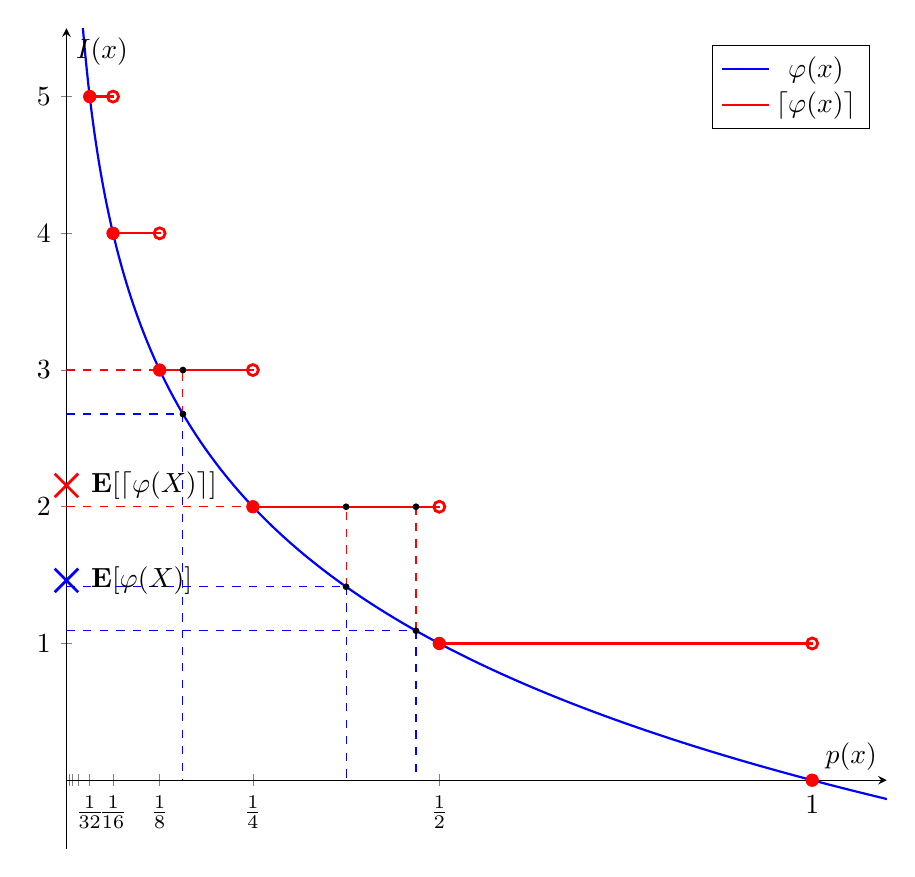
\begin{tikzpicture}
    \begin{axis}[
        domain=0.001:1.2,
        samples=1000,
        axis x line=middle,
        axis y line=middle,
        xlabel={$p(x)$},
        ylabel={$I(x)$},
        ymin=-0.5, ymax=5.5,
        xmin=0, xmax=1.1,
        height=12cm,
        width=12cm,
        xtick={1, 1/2, 1/4, 1/8, 1/16, 1/32, 1/64, 1/128, 1/256},
        xticklabels={$1$,
                     $\frac{1}{2}$,
                     $\frac{1}{4}$,
                     $\frac{1}{8}$,
                     $\frac{1}{16}$,
                     $\frac{1}{32}$},
    ]
        \addplot[thick,blue] {-(ln(x)/ln(2))};
        \addlegendentry{$\varphi(x)$}

        \addplot[thick,red,mark=none,domain=1/ 2:1/ 1] {1};
        \addplot[thick,red,mark=none,domain=1/ 4:1/ 2] {2};
        \addplot[thick,red,mark=none,domain=1/ 8:1/ 4] {3};
        \addplot[thick,red,mark=none,domain=1/16:1/ 8] {4};
        \addplot[thick,red,mark=none,domain=1/32:1/16] {5};
        \addplot[thick,red,mark=none,domain=1/64:1/32] {6};
        \addplot[only marks, mark=*, mark size=2.2pt, red] coordinates
        {(1/ 1, 0)
         (1/ 2, 1)
         (1/ 4, 2)
         (1/ 8, 3)
         (1/16, 4)
         (1/32, 5)};
        \addplot[only marks, mark=o, mark size=2pt, red, mark options={line width=1}] coordinates
        {(1/ 1, 1)
         (1/ 2, 2)
         (1/ 4, 3)
         (1/ 8, 4)
         (1/16, 5)};
        \addlegendentry{$\lceil \varphi(x) \rceil$}

        \addplot[only marks, mark=*, mark size=1pt, black] coordinates
        {( 5/32, 2.67807191)
         (12/32, 1.41503751)
         (15/32, 1.09310941)};

        \addplot[only marks, mark=*, mark size=1pt, black] coordinates
        {( 5/32, 3)
         (12/32, 2)
         (15/32, 2)};

        \draw[dashed,blue] ( 5/32, 2.67807191) -- ( 5/32,0);
        \draw[dashed,blue] (12/32, 1.41503751) -- (12/32,0);
        \draw[dashed,blue] (15/32, 1.09310941) -- (15/32,0);

        \draw[dashed,blue] (0, 2.67807191) -- ( 5/32, 2.67807191);
        \draw[dashed,blue] (0, 1.41503751) -- (12/32, 1.41503751);
        \draw[dashed,blue] (0, 1.09310941) -- (15/32, 1.09310941);

        \addplot[only marks, mark=x, mark size=6pt, blue, mark options={line width=1}] coordinates
        {(0, 1.46148)};
        \node[right] at (0.02, 1.46148) {$\mathbf E[\varphi(X)]$};

        \draw[dashed,red] ( 5/32, 2.67807191) -- ( 5/32,3);
        \draw[dashed,red] (12/32, 1.41503751) -- (12/32,2);
        \draw[dashed,red] (15/32, 1.09310941) -- (15/32,2);

        \draw[dashed,red] (0, 3) -- ( 5/32, 3);
        \draw[dashed,red] (0, 2) -- (12/32, 2);
        \draw[dashed,red] (0, 2) -- (15/32, 2);

        \addplot[only marks, mark=x, mark size=6pt, red, mark options={line width=1}] coordinates
        {(0, 2.15625)};
        \node[right] at (0.02, 2.15625) {$\mathbf E [\lceil \varphi(X) \rceil]$};

    \end{axis}
\end{tikzpicture}
\end{document}